% !TEX encoding = UTF-8 Unicode
% !TEX root = ../thesis.tex
% !TEX spellcheck = en-US
%%=========================================



\chapter{Results}\label{chap:results}




The results in this research project are mainly gathered from the final test session, which was held after the last development stage, thus the results reflect the state of the application at the end of the research. 

The test sessions had two separate quantitative data gathering strategies: 
A multiple choice knowledge test taken by the test participants before and after the session,  this was meant to demonstrate learning value in short term time frame. Such a simple short term test could support the claim that the artifact can be used as an educational tool. The test is attached as \autoref{chap:knowtest}.
The second strategy was a combined SUS questionnaire with general questions about the application. This questionnaire can be found as \autoref{chap:questionnaire}.
The knowledge test was taken by the medical students in test sessions, while the questionnaire was answered by six participants, of which four were medical students.

% though further research is needed.

\section{Neuroanatomical test}
The multiple choice neuroanatomical knowledge test was performed at both test sessions. The test was taken by three medical students at the first session, two third year and one fifth year student. At the second session five first year medical students partook in the knowledge test. The test was taken two times for each of the sessions; before using the IT artifact with lecturing from the neurologist, and then afterwards. \autoref{fig:knowtestres} shows the results from both test sessions, with blue bars indication the test taken before the session and red bars indicating the test taken after the session. In \autoref{chap:knowtest} all participant answers as well as the actual test with solution are provided.

\begin{figure}[H]
    \centering
    \begin{subfigure}[t]{0.8\textwidth}
        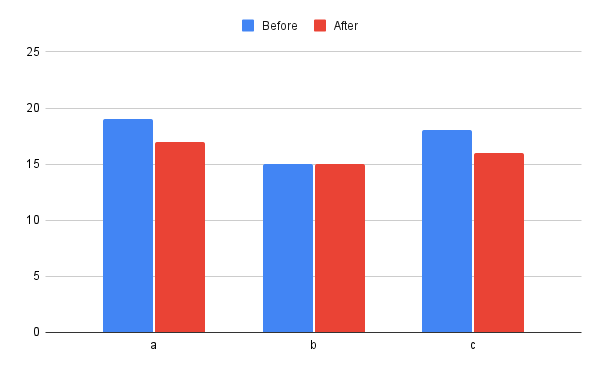
\includegraphics[width=\textwidth]{fig/knowtestresult1}
        \caption{First session}
    \end{subfigure}
    \begin{subfigure}[b]{0.8\textwidth}
        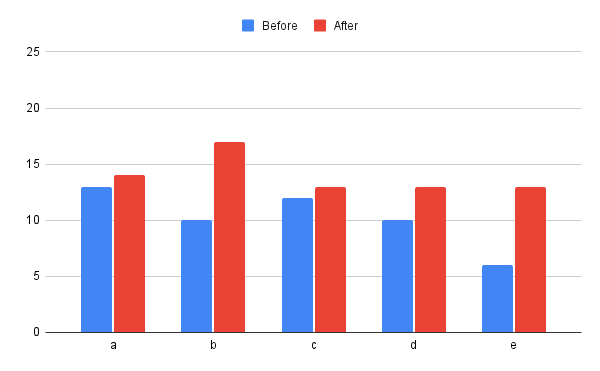
\includegraphics[width=\textwidth]{fig/knowtestresult2}
        \caption{Second session}
    \end{subfigure}
    \caption{Results from neuroanatomical knowledge test.}
    \label{fig:knowtestres}
\end{figure}





\section{Questionnaire}

The usability results are based on the second test session where a questionnaire, including a SUS section, was uses in addition to unstructured feedback from the test participants. The results from these methods will be presented in this section. 

\subsection{System usability scale questionnaire}
 
The SUS questionnaire was taken by six participants, five answering based on the HoloLens 2 experience and one based on using the Android application. The mean score from the HoloLens 2 is $79.0 \pm 10.4$, while the result from the single Android test was 75. This means that the application on HoloLens 2 sits high in the good rating almost reaching excellent, while the Android app is near the middle of the good rating. \autoref{fig:susresults} show the results of the SUS questionnaire charted with the red line representing the 68 \textit{average} score. All answers are listed in \autoref{tab:sus}, note that SUS is ordered such that every other statement is negative, meaning that a better score is achieved when they are disagreed to.

% Please add the following required packages to your document preamble:
% \usepackage[table,xcdraw]{xcolor}
% If you use beamer only pass "xcolor=table" option, i.e. \documentclass[xcolor=table]{beamer}
\begin{table}[]
    
\centering
\textbf{Results from SUS questionnaire}\par\medskip
\small
\begin{tabular}{l|ccccc}
\hline
                                                                                                                                         & \begin{tabular}[c]{@{}c@{}}Strongly\\ disagree\end{tabular} & Disagree                                                   & Neutral                                                    & Agree                                                     & \begin{tabular}[c]{@{}c@{}}Strongly\\ agree\end{tabular}   \\ \hline
\begin{tabular}[c]{@{}l@{}}I think that I would like to use this \\ system frequently.\end{tabular}                                      & {\color[HTML]{333333} \textbf{}}                            & {\color[HTML]{333333} \textbf{}}                           & {\color[HTML]{333333} \textbf{}}                           & \cellcolor[HTML]{9698ED}{\color[HTML]{EFEFEF} \textbf{2}} & \cellcolor[HTML]{6434FC}{\color[HTML]{EFEFEF} \textbf{4*}} \\
\rowcolor[HTML]{EFEFEF} 
\begin{tabular}[c]{@{}l@{}}I found the system \\ unnecessarily complex.\end{tabular}                                                     & \cellcolor[HTML]{6665CD}{\color[HTML]{EFEFEF} \textbf{3}}   & \cellcolor[HTML]{9698ED}{\color[HTML]{EFEFEF} \textbf{2*}} & \cellcolor[HTML]{CBCEFB}{\color[HTML]{EFEFEF} \textbf{1}}  & {\color[HTML]{333333} \textbf{}}                          & {\color[HTML]{333333} \textbf{}}                           \\
\begin{tabular}[c]{@{}l@{}}I thought the system was \\ easy to use.\end{tabular}                                                         & {\color[HTML]{333333} \textbf{}}                            & {\color[HTML]{333333} \textbf{}}                           & \cellcolor[HTML]{9698ED}{\color[HTML]{EFEFEF} \textbf{2*}} & \cellcolor[HTML]{6434FC}{\color[HTML]{EFEFEF} \textbf{4}} & {\color[HTML]{333333} \textbf{}}                           \\
\rowcolor[HTML]{EFEFEF} 
\begin{tabular}[c]{@{}l@{}}I think that I would need the \\ support of a technical person \\ to be able to use this system.\end{tabular} & \cellcolor[HTML]{6665CD}{\color[HTML]{EFEFEF} \textbf{3*}}  & \cellcolor[HTML]{9698ED}{\color[HTML]{EFEFEF} \textbf{2}}  & \cellcolor[HTML]{CBCEFB}{\color[HTML]{EFEFEF} \textbf{1}}  & {\color[HTML]{333333} \textbf{}}                          & {\color[HTML]{333333} \textbf{}}                           \\
\begin{tabular}[c]{@{}l@{}}I found the various functions in \\ this system were well integrated.\end{tabular}                            & {\color[HTML]{333333} \textbf{}}                            & {\color[HTML]{333333} \textbf{}}                           & \cellcolor[HTML]{CBCEFB}{\color[HTML]{EFEFEF} \textbf{1*}} & \cellcolor[HTML]{6434FC}{\color[HTML]{EFEFEF} \textbf{4}} & \cellcolor[HTML]{CBCEFB}{\color[HTML]{EFEFEF} \textbf{1}}  \\
\cellcolor[HTML]{EFEFEF}\begin{tabular}[c]{@{}l@{}}I thought there was too much \\ inconsistency in this system.\end{tabular}            & \cellcolor[HTML]{CBCEFB}{\color[HTML]{EFEFEF} \textbf{1}}   & \cellcolor[HTML]{6665CD}{\color[HTML]{EFEFEF} \textbf{3}}  & \cellcolor[HTML]{CBCEFB}{\color[HTML]{EFEFEF} \textbf{1}}  & \cellcolor[HTML]{CBCEFB}{\color[HTML]{EFEFEF} \textbf{1*}}   & \cellcolor[HTML]{EFEFEF}\textbf{}                          \\
\begin{tabular}[c]{@{}l@{}}I would imagine that most \\ people would learn to use \\ this system very quickly.\end{tabular}              & {\color[HTML]{333333} \textbf{}}                            & {\color[HTML]{333333} \textbf{}}                           & \cellcolor[HTML]{CBCEFB}{\color[HTML]{EFEFEF} \textbf{1}}  & \cellcolor[HTML]{6665CD}{\color[HTML]{EFEFEF} \textbf{3}} & \cellcolor[HTML]{9698ED}{\color[HTML]{EFEFEF} \textbf{2*}} \\
\rowcolor[HTML]{EFEFEF} 
\begin{tabular}[c]{@{}l@{}}I found the system very \\ cumbersome to use.\end{tabular}                                                    & \cellcolor[HTML]{9698ED}{\color[HTML]{EFEFEF} \textbf{2}}   & \cellcolor[HTML]{6665CD}{\color[HTML]{EFEFEF} \textbf{3}}  & \cellcolor[HTML]{CBCEFB}{\color[HTML]{EFEFEF} \textbf{1*}} & {\color[HTML]{333333} \textbf{}}                          & {\color[HTML]{333333} \textbf{}}                           \\
\begin{tabular}[c]{@{}l@{}}I felt very confident using \\ the system.\end{tabular}                                                       & {\color[HTML]{333333} \textbf{}}                            & {\color[HTML]{333333} \textbf{}}                           & \cellcolor[HTML]{CBCEFB}{\color[HTML]{EFEFEF} \textbf{1}}  & \cellcolor[HTML]{9698ED}{\color[HTML]{EFEFEF} \textbf{2}} & \cellcolor[HTML]{6665CD}{\color[HTML]{EFEFEF} \textbf{3*}} \\
\rowcolor[HTML]{EFEFEF} 
\begin{tabular}[c]{@{}l@{}}I needed to learn a lot of \\ things before I could get \\ going with this system.\end{tabular}               & \cellcolor[HTML]{9698ED}{\color[HTML]{EFEFEF} \textbf{2*}}  & \cellcolor[HTML]{6665CD}{\color[HTML]{EFEFEF} \textbf{3}}  & {\color[HTML]{333333} \textbf{}}                           & \cellcolor[HTML]{CBCEFB}{\color[HTML]{EFEFEF} \textbf{1}} & {\color[HTML]{333333} \textbf{}}                           \\ \hline
\end{tabular}
\caption{The results form the SUS section. Number and color values represent the magnitude of answers with the corresponding alternative. Android answer is marked with "*".}
\label{tab:sus}

\end{table}

\begin{figure}
    \centering
    \textbf{SUS results}\par\medskip
    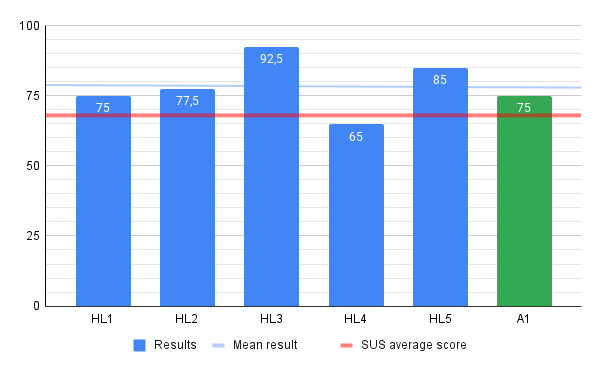
\includegraphics[width=0.75\textwidth]{fig/susbarchart}
    \caption{The blue results are from HoloLens 2, while the green is from Android.}
    \label{fig:susresults}
\end{figure}


\subsection{Research specific questionnaire}\label{chap:researchspes}
The questionnaire included a section with research specific questions written by the researcher with the aim to gather data relating to the research questions of the project. The question were, just as in SUS, based on the \textit{Likert scale}, with answer alternatives ranging from 1 - 5 indicating how much in agreement the user is with the statement. The section was answered by six participants, and it was platform independent. The results can be seen in \autoref{tab:researchspes}. In addition to the Likert ranking free form text boxes were provided after the questions for gathering qualitative data. 


% Notably, the participants were asked what platform they preferred
Notably, every participant who tried both platforms preferred the HoloLens 2 experience, based on the question \textit{Which platform did you prefer?}. Saying the following:
\newline

{\small
\noindent
\textbf{Why did you prefer that platform?}
\begin{itemize}[]
    \itshape\footnotesize
    \item Physically interactive and the menu is on your hand
    \item Much easier to understand the 3d structure, as you can see and rotate it at any angle.
    \item Holo is easier to manoeuvre and look from different angles.
    \item It was more a more fun way of learning, which again increases motivation for learning.
\end{itemize}
}
\noindent
Addition questions with free text input were answered as follow:
\newline

{\small
\noindent
\textbf{Please explain if you learned something or why you feel you did not.}
\begin{itemize}[]
    \itshape\footnotesize
    \item I learned about the three dimensional placement of structures in the brain and how the structures are placed relatively to each other
    \item I did learn something. Got a new perspective
    \item I learned the 3d structural layout that goes along with the regions and labels we use. However, for someone without any prior knowledge of the brains substructures, it would be a lot of information, both visual and names of regions.
    \item Knew very little before comming, and learned a little bit while watching the other explore and exploring myself. I think it helped having Menno there to point parts out and ask questions.
    \item I feel I learned more about the anatomy of the rodent brain while picking it apart and puzzling it back together. However I wish I had morr time to read the description of the different brain parts as well.
\end{itemize}
}

{\small
\noindent
\textbf{Please explain how you feel collaboration was facilitated in the system.}
\begin{itemize}[]
    \itshape\footnotesize

\item The ability to see the parts that were moved by the others and their pointer. Also the synchronization was helpfull
    It was a bit difficult to see what the other person was doing, but it was very fun when verbally communicating with that other person.
   \item Due to some bug, I was unable to see the other persons pointer.
    Didnt work very well in our test. I quickly got messy with multiple people manipulating the brain
    \item Lagged a bit and smal difficulties moving the brain around to the position one wants.
   \item Did not try collaboration that much. Was mostly getting familliar with the system, so did not focus on the fact that it was possible to collaborate to learn toghether and explore toghether.


\end{itemize}
}

{\small
\noindent
\textbf{Do you have other thoughts about the Nevrolens application. Feel free to write any feedback or insight here.}
\begin{itemize}[]
    \itshape\footnotesize
    \item I think it could be benifitial to have an initial «tutorial» to make it easier for users to get to know the application in the beginning. Maybe also naming of different parts during dissection
    \item Great Experience. Enjoyable to interact with the 3d Brain
    \item This is a great system promoting learning.


\end{itemize}
}
% Please add the following required packages to your document preamble:
% \usepackage[table,xcdraw]{xcolor}
% If you use beamer only pass "xcolor=table" option, i.e. \documentclass[xcolor=table]{beamer}
% \usepackage[normalem]{ulem}
% \useunder{\uline}{\ul}{}
\begin{table}[h]
\centering
\textbf{Results from research questionnaire}\par\medskip
\small
\begin{tabular}{l|ccccc}
\hline
                                                                                                                                                          & \begin{tabular}[c]{@{}c@{}}Strongly\\ disagree\end{tabular} & Disagree                                                  & Neutral                                                   & Agree                                                     & \begin{tabular}[c]{@{}c@{}}Strongly\\ agree\end{tabular}  \\ \hline
\begin{tabular}[c]{@{}l@{}}I got new insight about neuroanatomy \\ while using the system.\end{tabular}                                                   & \textbf{}                                                   & \textbf{}                                                 & \textbf{}                                                 & \cellcolor[HTML]{6434FC}{\color[HTML]{EFEFEF} \textbf{4}} & \cellcolor[HTML]{9698ED}{\color[HTML]{EFEFEF} \textbf{2}} \\
\rowcolor[HTML]{EFEFEF} 
\begin{tabular}[c]{@{}l@{}}I got new insight about neuroanatomy \\ while seeing and manipulating the \\ brain and its structures in 3D.\end{tabular}      & \textbf{}                                                   & \textbf{}                                                 & \textbf{}                                                 & \cellcolor[HTML]{9698ED}{\color[HTML]{EFEFEF} \textbf{2}} & \cellcolor[HTML]{6434FC}{\color[HTML]{EFEFEF} \textbf{4}} \\
\begin{tabular}[c]{@{}l@{}}I got new insight about neuroanatomy \\ while dissecting the brain.\end{tabular}                                               & \textbf{}                                                   & \textbf{}                                                 & \cellcolor[HTML]{CBCEFB}{\color[HTML]{EFEFEF} \textbf{1}} & \cellcolor[HTML]{6200C9}{\color[HTML]{EFEFEF} \textbf{5}} & \textbf{}                                                 \\
\rowcolor[HTML]{EFEFEF} 
\cellcolor[HTML]{EFEFEF}\begin{tabular}[c]{@{}l@{}}I felt like I was collaborating with another \\ person when using the system with others.\end{tabular} & \cellcolor[HTML]{CBCEFB}{\color[HTML]{EFEFEF} \textbf{1}}                           & \cellcolor[HTML]{CBCEFB}{\color[HTML]{EFEFEF} \textbf{1}}                         & \cellcolor[HTML]{6665CD}{\color[HTML]{EFEFEF} \textbf{3}} & \cellcolor[HTML]{CBCEFB}{\color[HTML]{EFEFEF} \textbf{1}}                         & \cellcolor[HTML]{EFEFEF}\textbf{}                         \\
\begin{tabular}[c]{@{}l@{}}I was aware of what the other person did \\ and had focus on when using the system.\end{tabular}                               & \textbf{}                                                   & \cellcolor[HTML]{9698ED}{\color[HTML]{EFEFEF} \textbf{2}} & \cellcolor[HTML]{6665CD}{\color[HTML]{EFEFEF} \textbf{3}} & \cellcolor[HTML]{CBCEFB}{\color[HTML]{EFEFEF} \textbf{1}} & \textbf{}                                                 \\
\rowcolor[HTML]{EFEFEF} 
\begin{tabular}[c]{@{}l@{}}The system would be useful for remote \\ teaching of neuroanatomy.\end{tabular}                                                & \textbf{}                                                   & \textbf{}                                                 & \cellcolor[HTML]{CBCEFB}{\color[HTML]{EFEFEF} \textbf{1}} & \cellcolor[HTML]{9698ED}{\color[HTML]{EFEFEF} \textbf{2}} & \cellcolor[HTML]{6665CD}{\color[HTML]{EFEFEF} \textbf{3}} \\ \hline
\end{tabular}
\caption{The results form the research specific questions, the number and color values represent the magnitude of answers with the corresponding alternative.}
\label{tab:researchspes}
\end{table}

\subsection{IPEAR AR and peer learning questionnaire}
This section was included as part of other research at the NTNU VRLab. The results from the section is however just as relevant for this study. \autoref{tab:peer} shows the results. Free form text answer where given to as are provided bellow. In this section those questions are modified for clarity as in the questionnaire free form question was a "Why?" as a follow up to the previous Likert scale question. For more detail \autoref{chap:questionnaire} has all answers unformatted.
\newline

{\small
\noindent
\textbf{Did you like the approach of peer learning (working with and teaching your classmates)? Why?}
\begin{itemize}[]
    \itshape\footnotesize


\item You can share knowledge and discuss facts to furter solidify the theory
\item Learning alongside others is very fun, especially after having had remote electronic learning.
    \item Personal preference
    \item Because it is interactive and communicative.


\end{itemize}
}

{\small
\noindent
\textbf{Were you more interested in teaching each other and sharing content with your peers and AR tools? Why?}
\begin{itemize}[]
    \itshape\footnotesize
    \item It was exciting to try the technology with a classmate and it gave a new dimension to the cooperation
    \item Because it was fun and interesting
    \item Didnt feel it
    \item Because this is a great new way of teaching and learning.


\end{itemize}
}
\begin{table}[]
\centering
\textbf{Results from AR and peer learning questionnaire}\par\medskip
\small
\begin{tabular}{l|ccccc}
\hline
                                                                                                                                             & \begin{tabular}[c]{@{}c@{}}Strongly\\ disagree\end{tabular} & Disagree                                                  & Neutral                                                   & Agree                                                     & \begin{tabular}[c]{@{}c@{}}Strongly\\ agree\end{tabular}  \\ \hline
\begin{tabular}[c]{@{}l@{}}Did you like the approach of peer learning \\ \small{(working with and teaching your classmates)}?\end{tabular}           & \textbf{}                                                   & \textbf{}                                                 & \cellcolor[HTML]{6665CD}{\color[HTML]{EFEFEF} \textbf{3}} &  & \cellcolor[HTML]{6665CD}{\color[HTML]{EFEFEF} \textbf{3}} \\
\rowcolor[HTML]{EFEFEF} 
\begin{tabular}[c]{@{}l@{}}Were you more interested in teaching \\each other  and sharing content with \\your peers and AR tools?\end{tabular} & \textbf{}                                                   & \cellcolor[HTML]{CBCEFB}{\color[HTML]{EFEFEF} \textbf{1}} & \cellcolor[HTML]{CBCEFB}{\color[HTML]{EFEFEF} \textbf{1}} & \cellcolor[HTML]{6434FC}{\color[HTML]{EFEFEF} \textbf{4}} & {\color[HTML]{EFEFEF} \textbf{}}                          \\
\begin{tabular}[c]{@{}l@{}}Did this learning approach make you feel \\ more responsible for your learning?\end{tabular}                      & \textbf{}                                                   & \cellcolor[HTML]{CBCEFB}{\color[HTML]{EFEFEF} \textbf{1}} & \cellcolor[HTML]{6665CD}{\color[HTML]{EFEFEF} \textbf{3}} & \cellcolor[HTML]{CBCEFB}{\color[HTML]{EFEFEF} \textbf{1}} & \cellcolor[HTML]{CBCEFB}{\color[HTML]{EFEFEF} \textbf{1}} \\
\rowcolor[HTML]{EFEFEF} 
\begin{tabular}[c]{@{}l@{}}Do you think it would be useful in other \\ courses or fields of study as well?\end{tabular}                      & {\color[HTML]{EFEFEF} \textbf{}}                            & {\color[HTML]{EFEFEF} \textbf{}}                          & {\color[HTML]{EFEFEF} \textbf{}}                          & \cellcolor[HTML]{9698ED}{\color[HTML]{EFEFEF} \textbf{2}} & \cellcolor[HTML]{6434FC}{\color[HTML]{EFEFEF} \textbf{4}} \\ \hline
\end{tabular}
\caption{The results form the research specific questions, the number and color values represent the magnitude of answers with the corresponding alternative.}
\label{tab:peer}
\end{table}


\subsection{Feedback from participants}

During the test sessions the participants gave feedback on their thoughts of the application, and how to improve the user experience. For the HoloLens 2 application the stated feedback was overwhelmingly positive, in \autoref{chap:researchspes} some give more constructive feedback which was not pointed out when talking with the participants. For the Android experience the prime vocalized feedback was to disable the AR in the application such that it would be a standard 3D application, this was explained both by the poor spatial locking on the device and the non optimal ergonomics of having to point the camera on the same spot at all times. 





%====================================================

% % The result of this project is the preliminary work for my master thesis next semester, thus 

% \section{Nevrolens}\label{nevrolens}
% Nevrolens is the name I've given the application which is the research product of this project. It's a combination of the Norwegian word Nevroanatomi and HoloLens. It is a AR application running on HoloLens 1, HoloLens 2 and Android. 

% The application is focused on delivering a single user experience, with features as cutting planes, scaling, moving brain parts and transparent brain parts. \autoref{fig:nevrolens_holo} show these features running on HoloLens 2, while \autoref{fig:nevrolens_android} show them on Android.
% It is packages and released on GitLab at \url{https://gitlab.stud.idi.ntnu.no/imtel/nevrolens}. 

% \begin{figure}[h]\label{fig:nevrolens_holo}
%     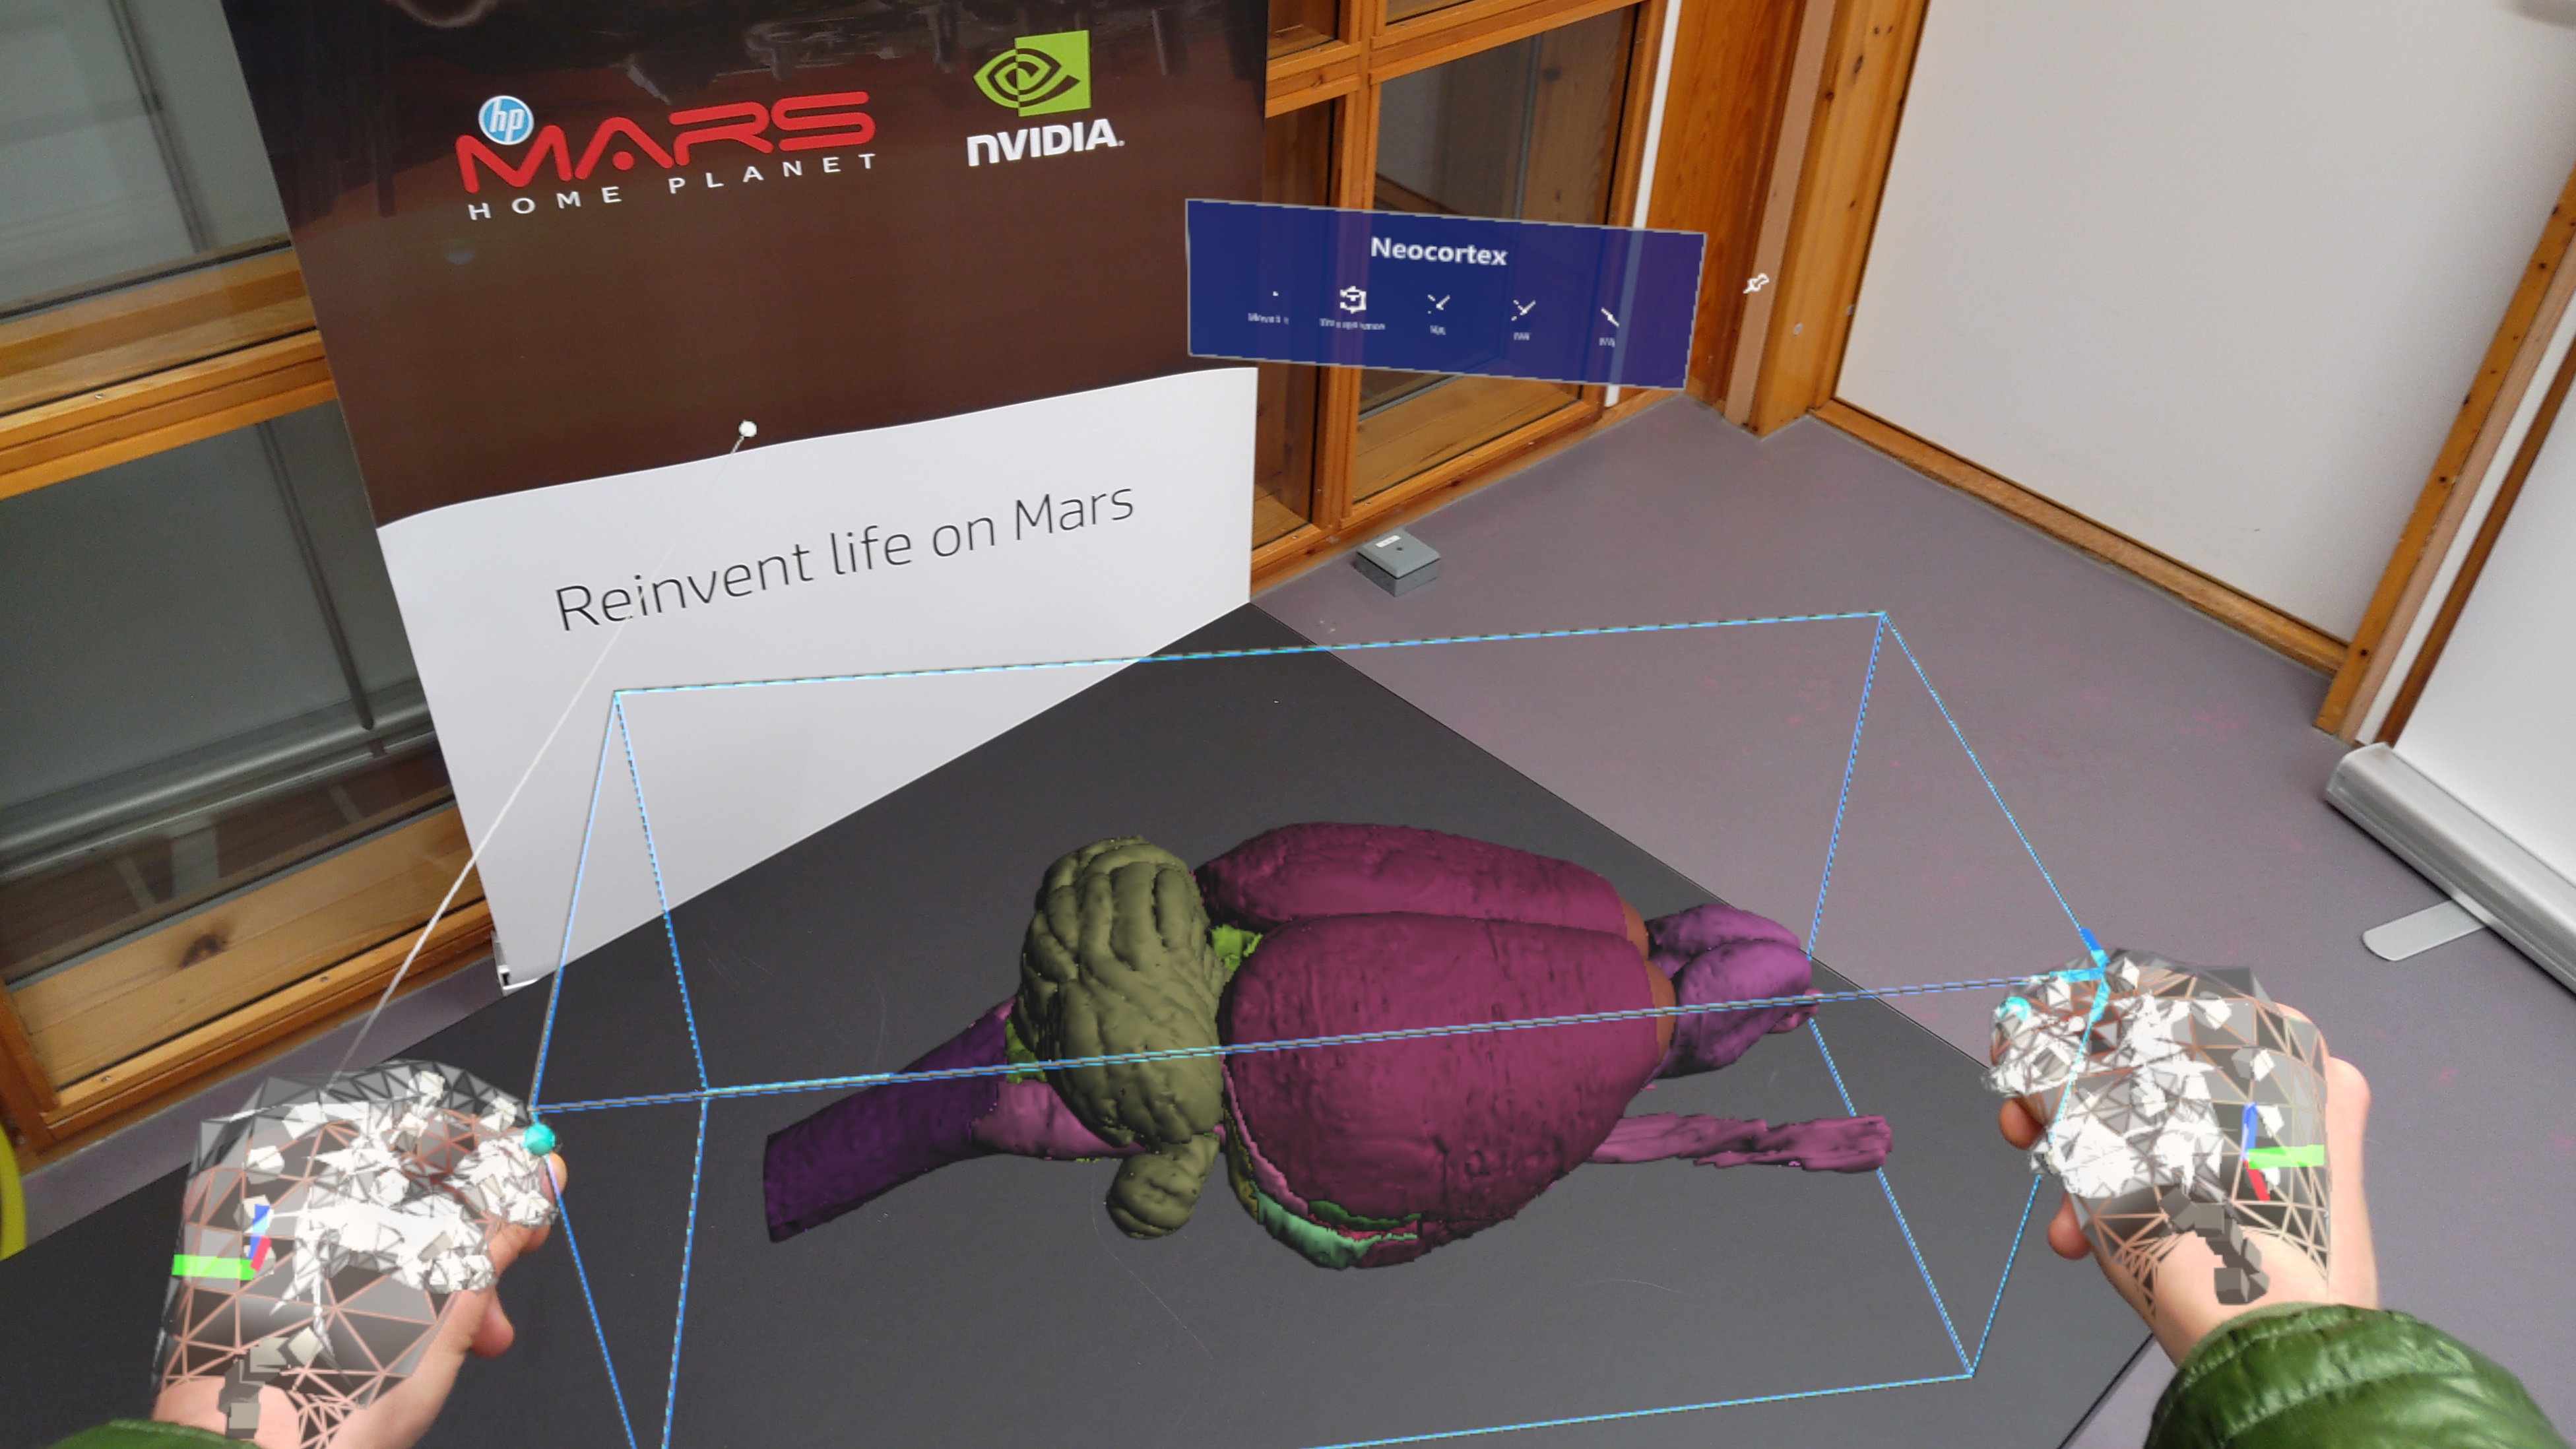
\includegraphics[width=0.5\textwidth]{fig/nevrolens/twohandedzoom.jpg}
%     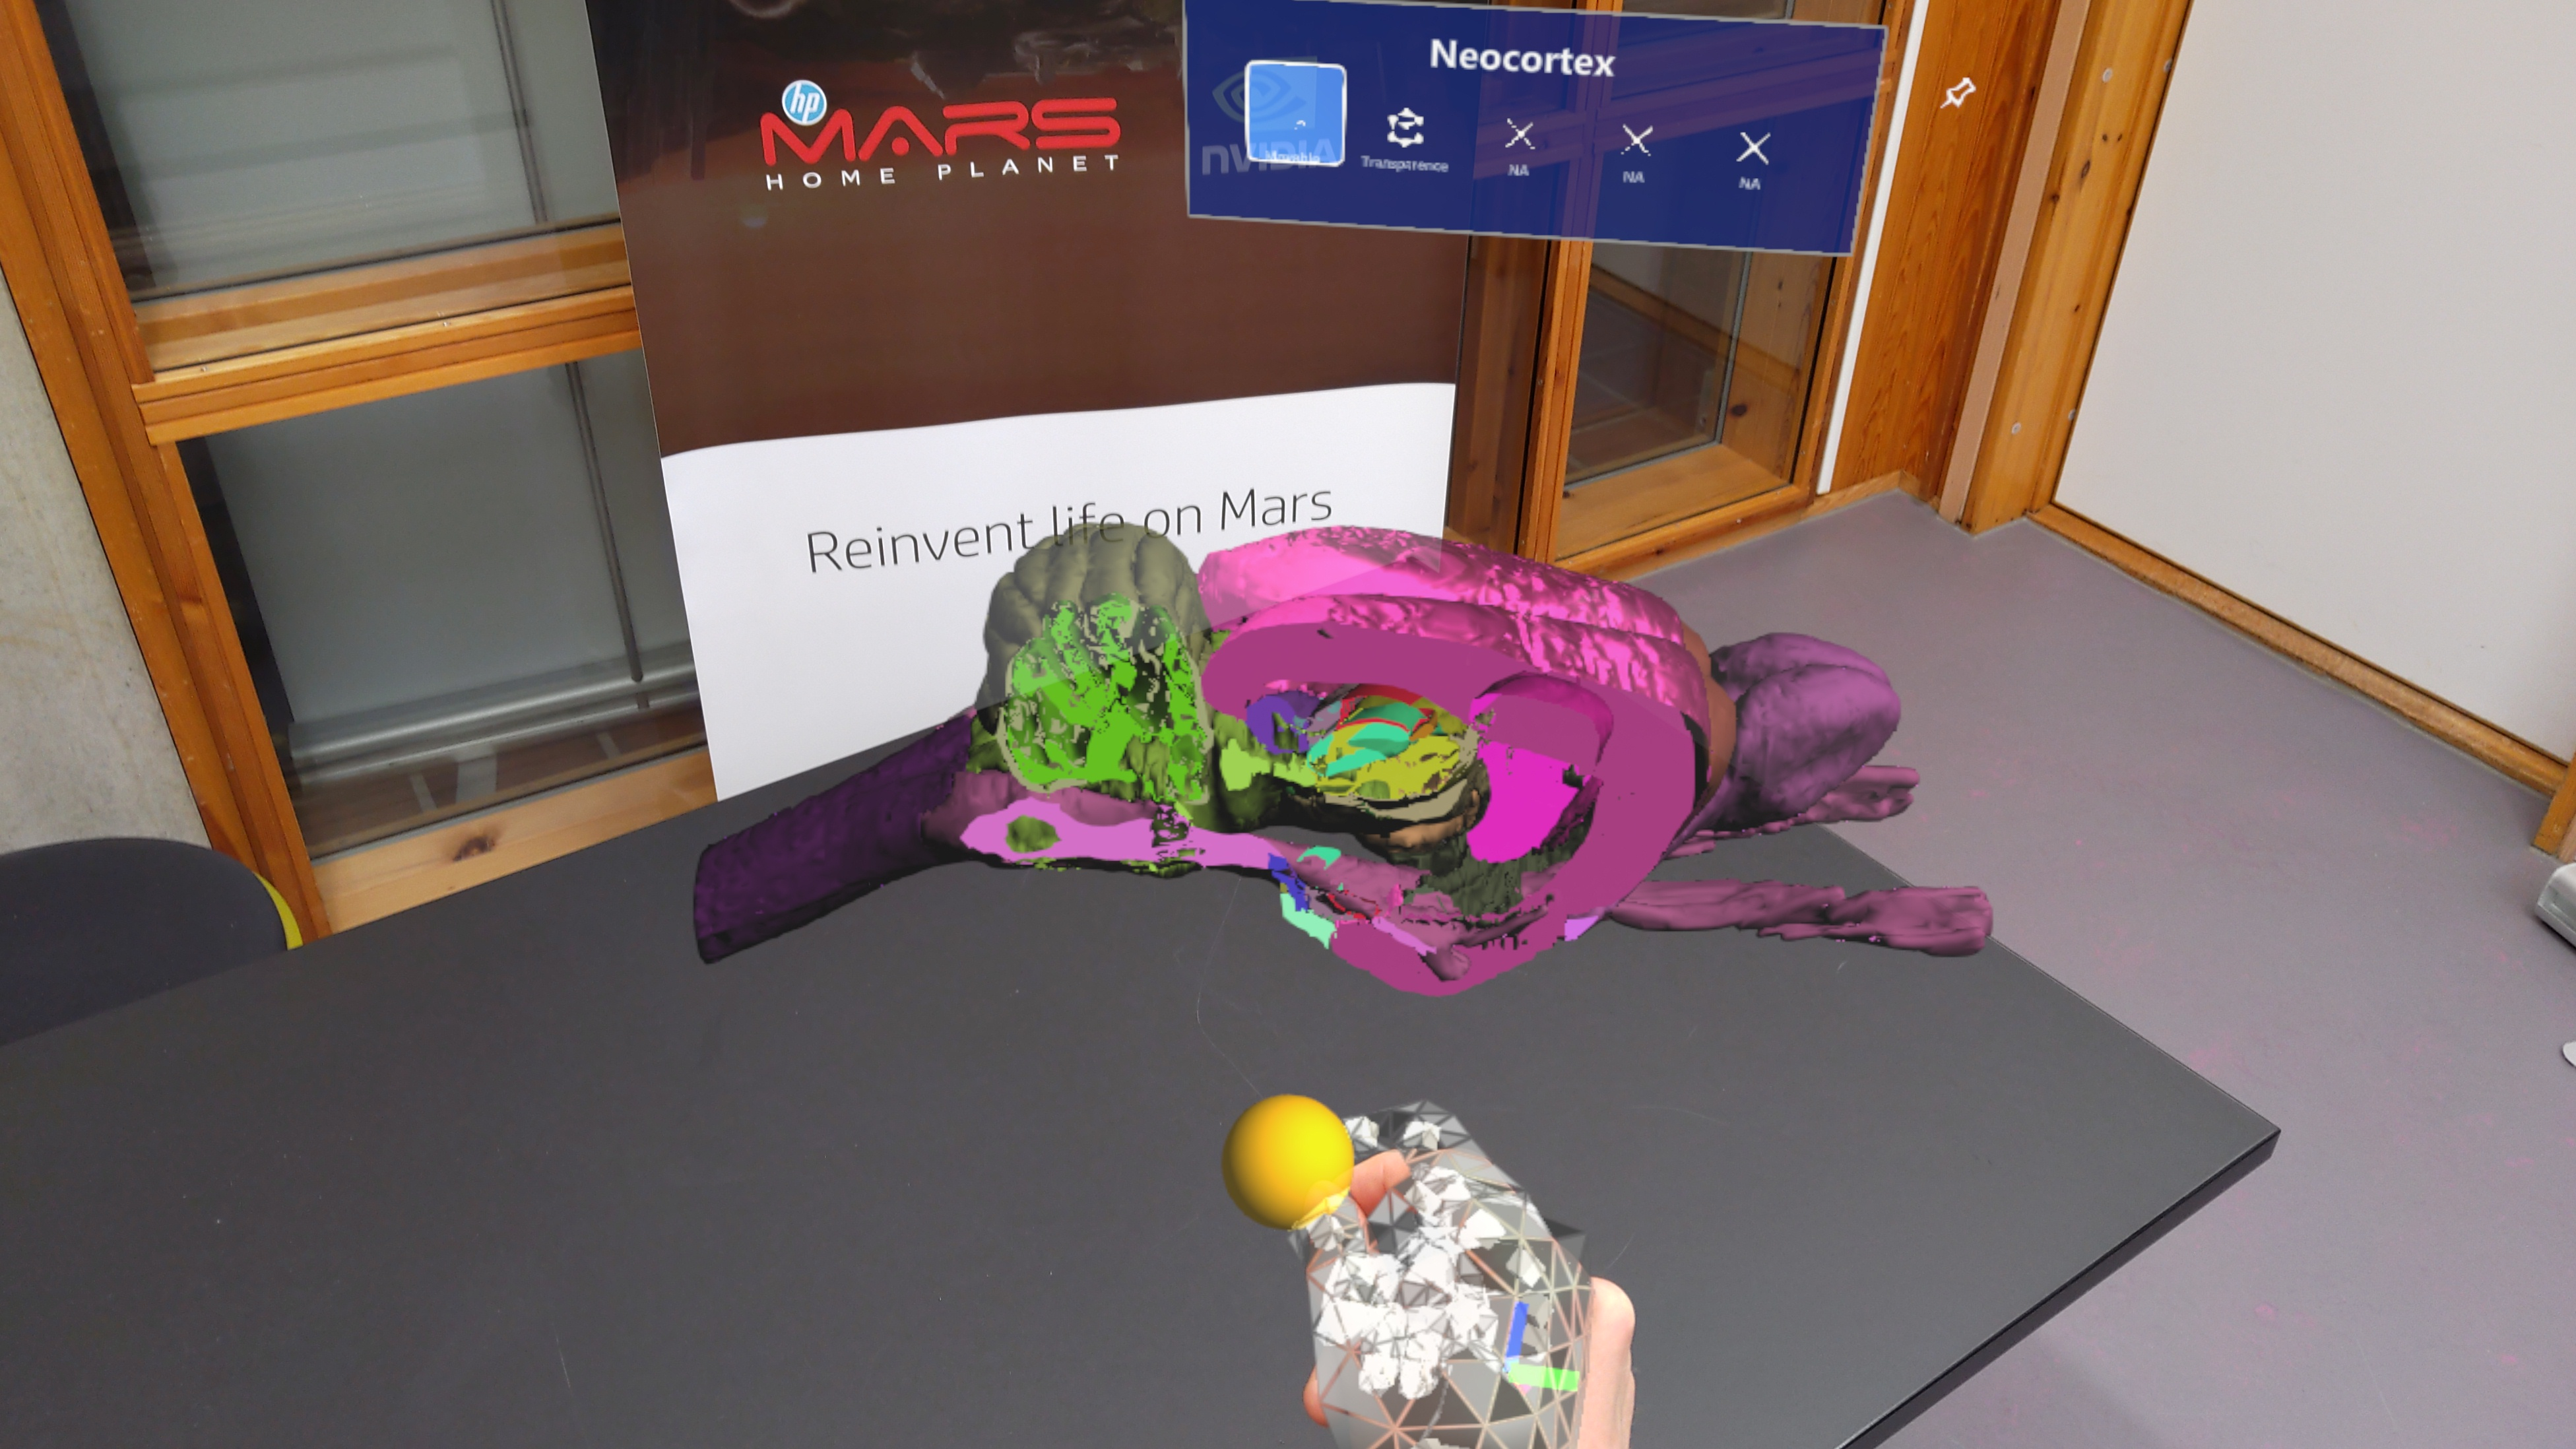
\includegraphics[width=0.5\textwidth]{fig/nevrolens/clipping.jpg}
%     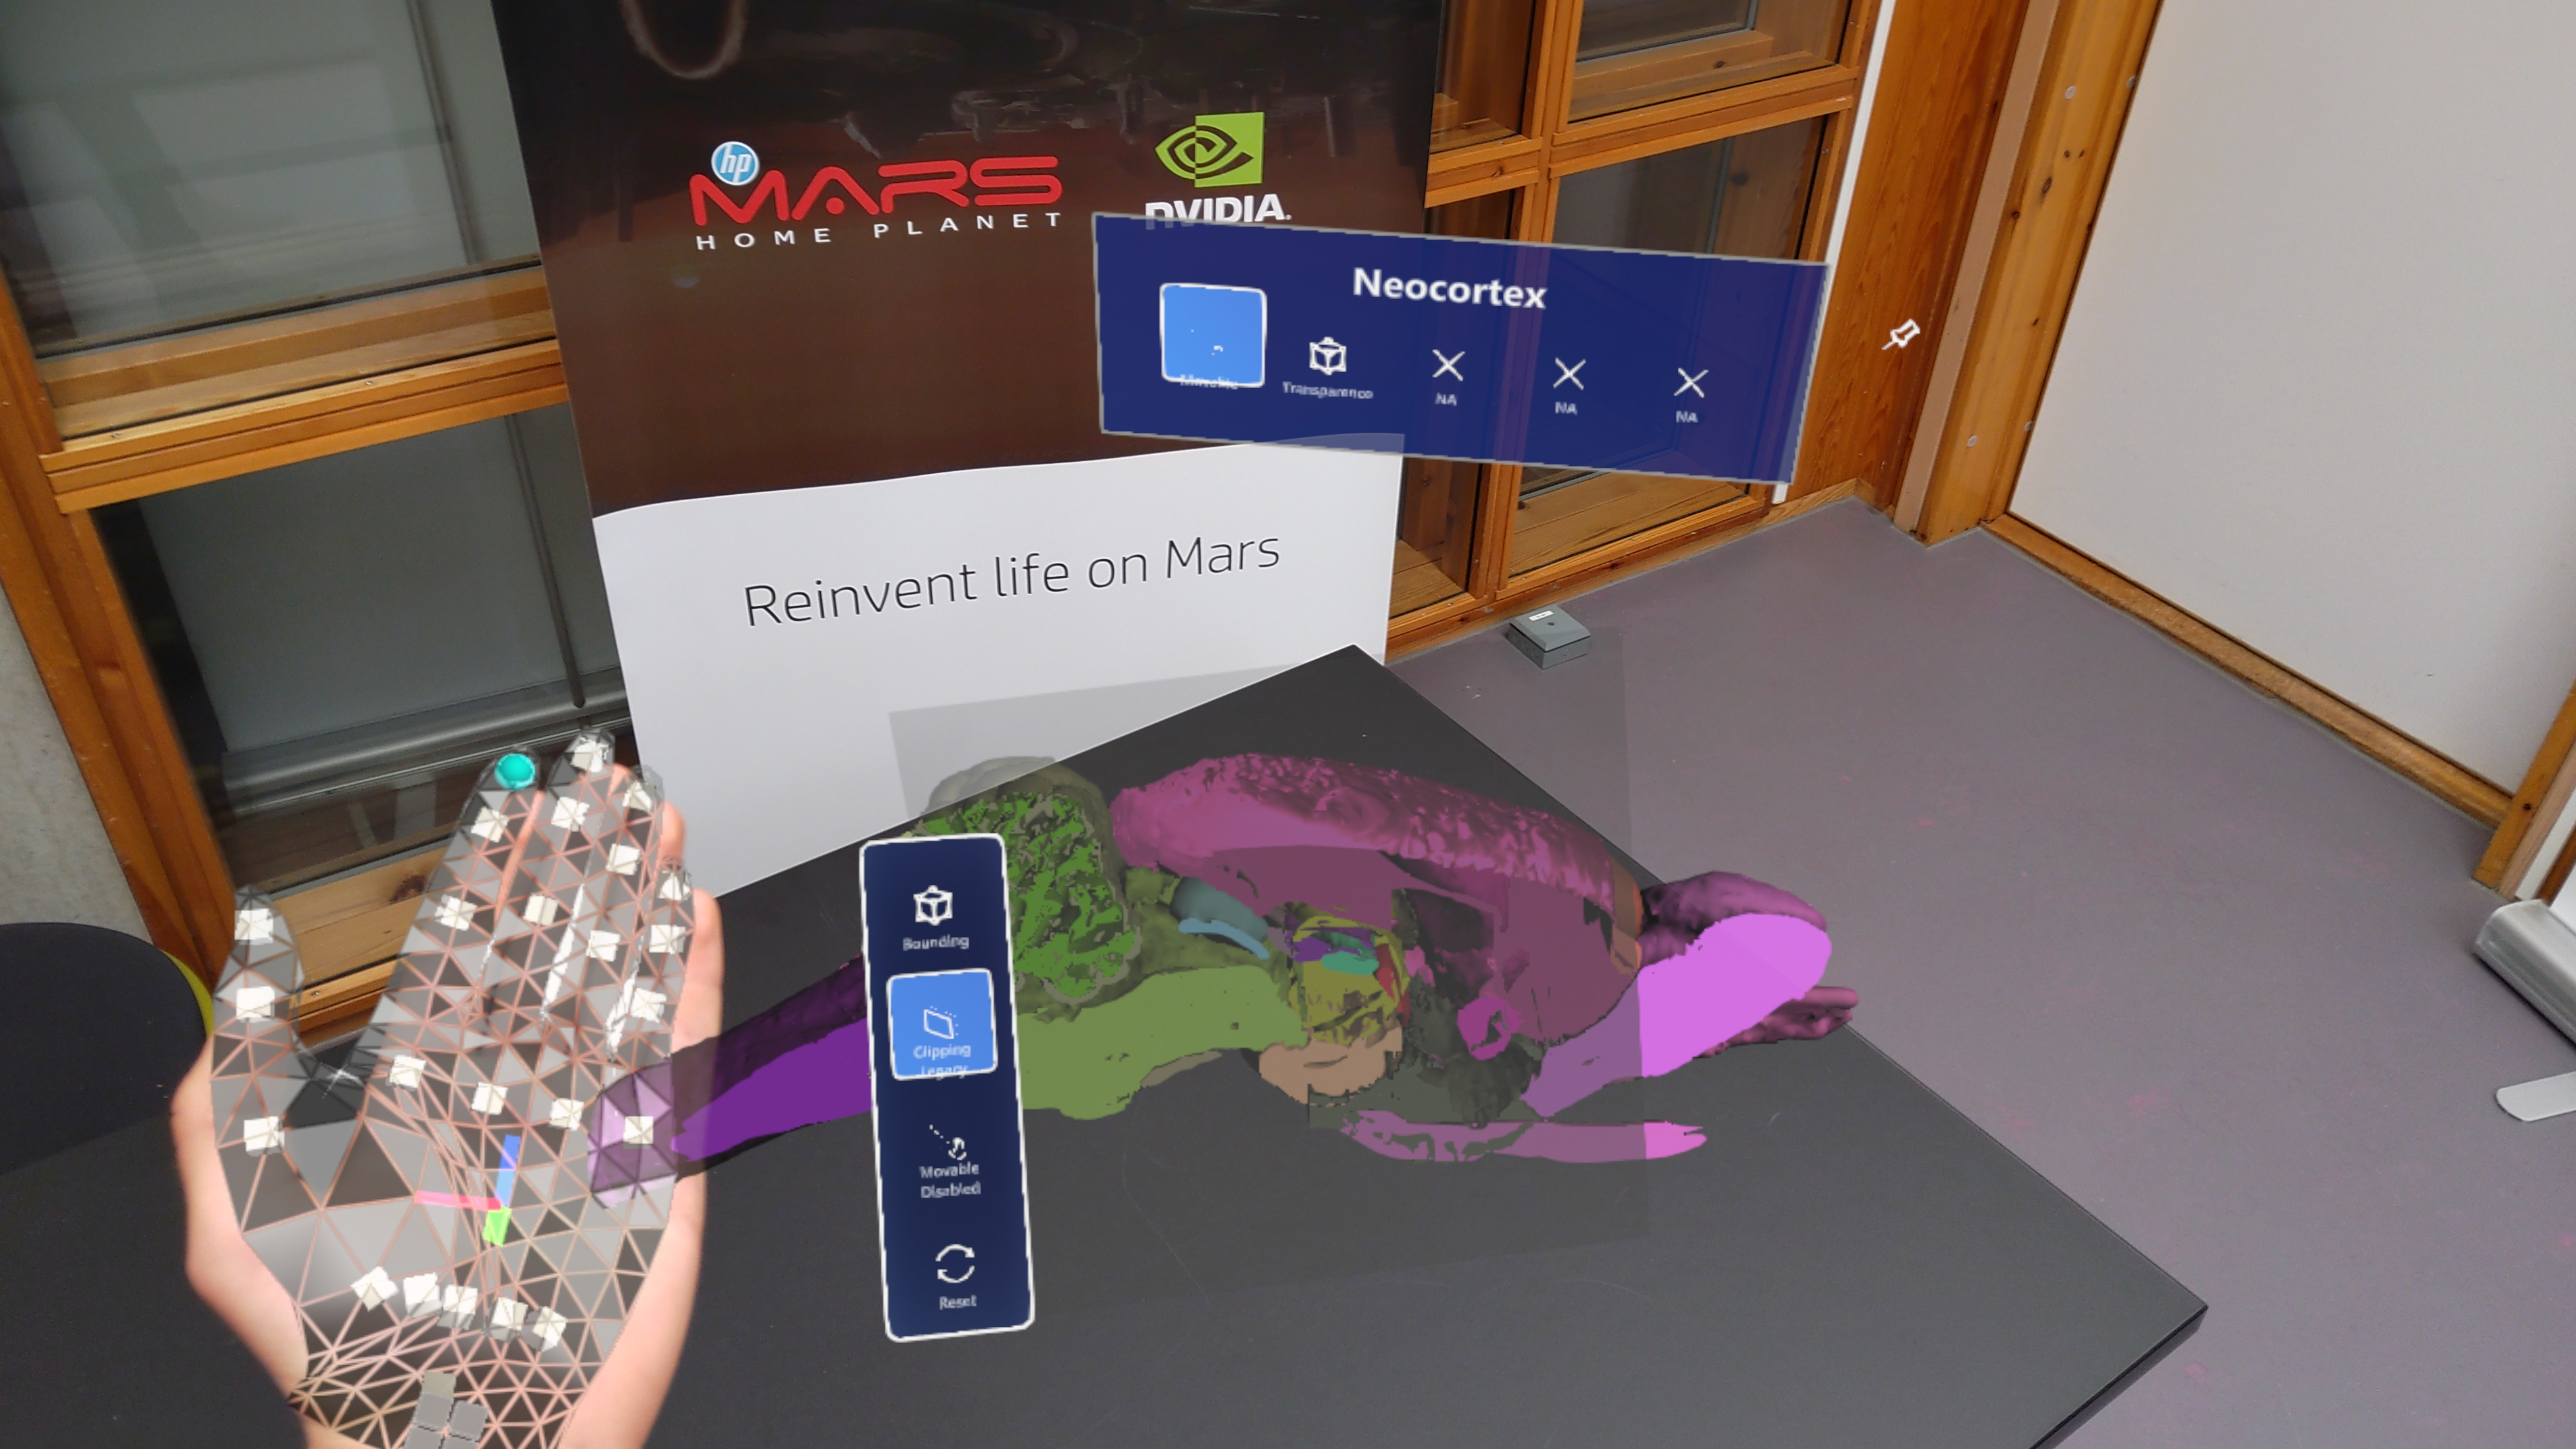
\includegraphics[width=0.5\textwidth]{fig/nevrolens/palmmenu.jpg}
%     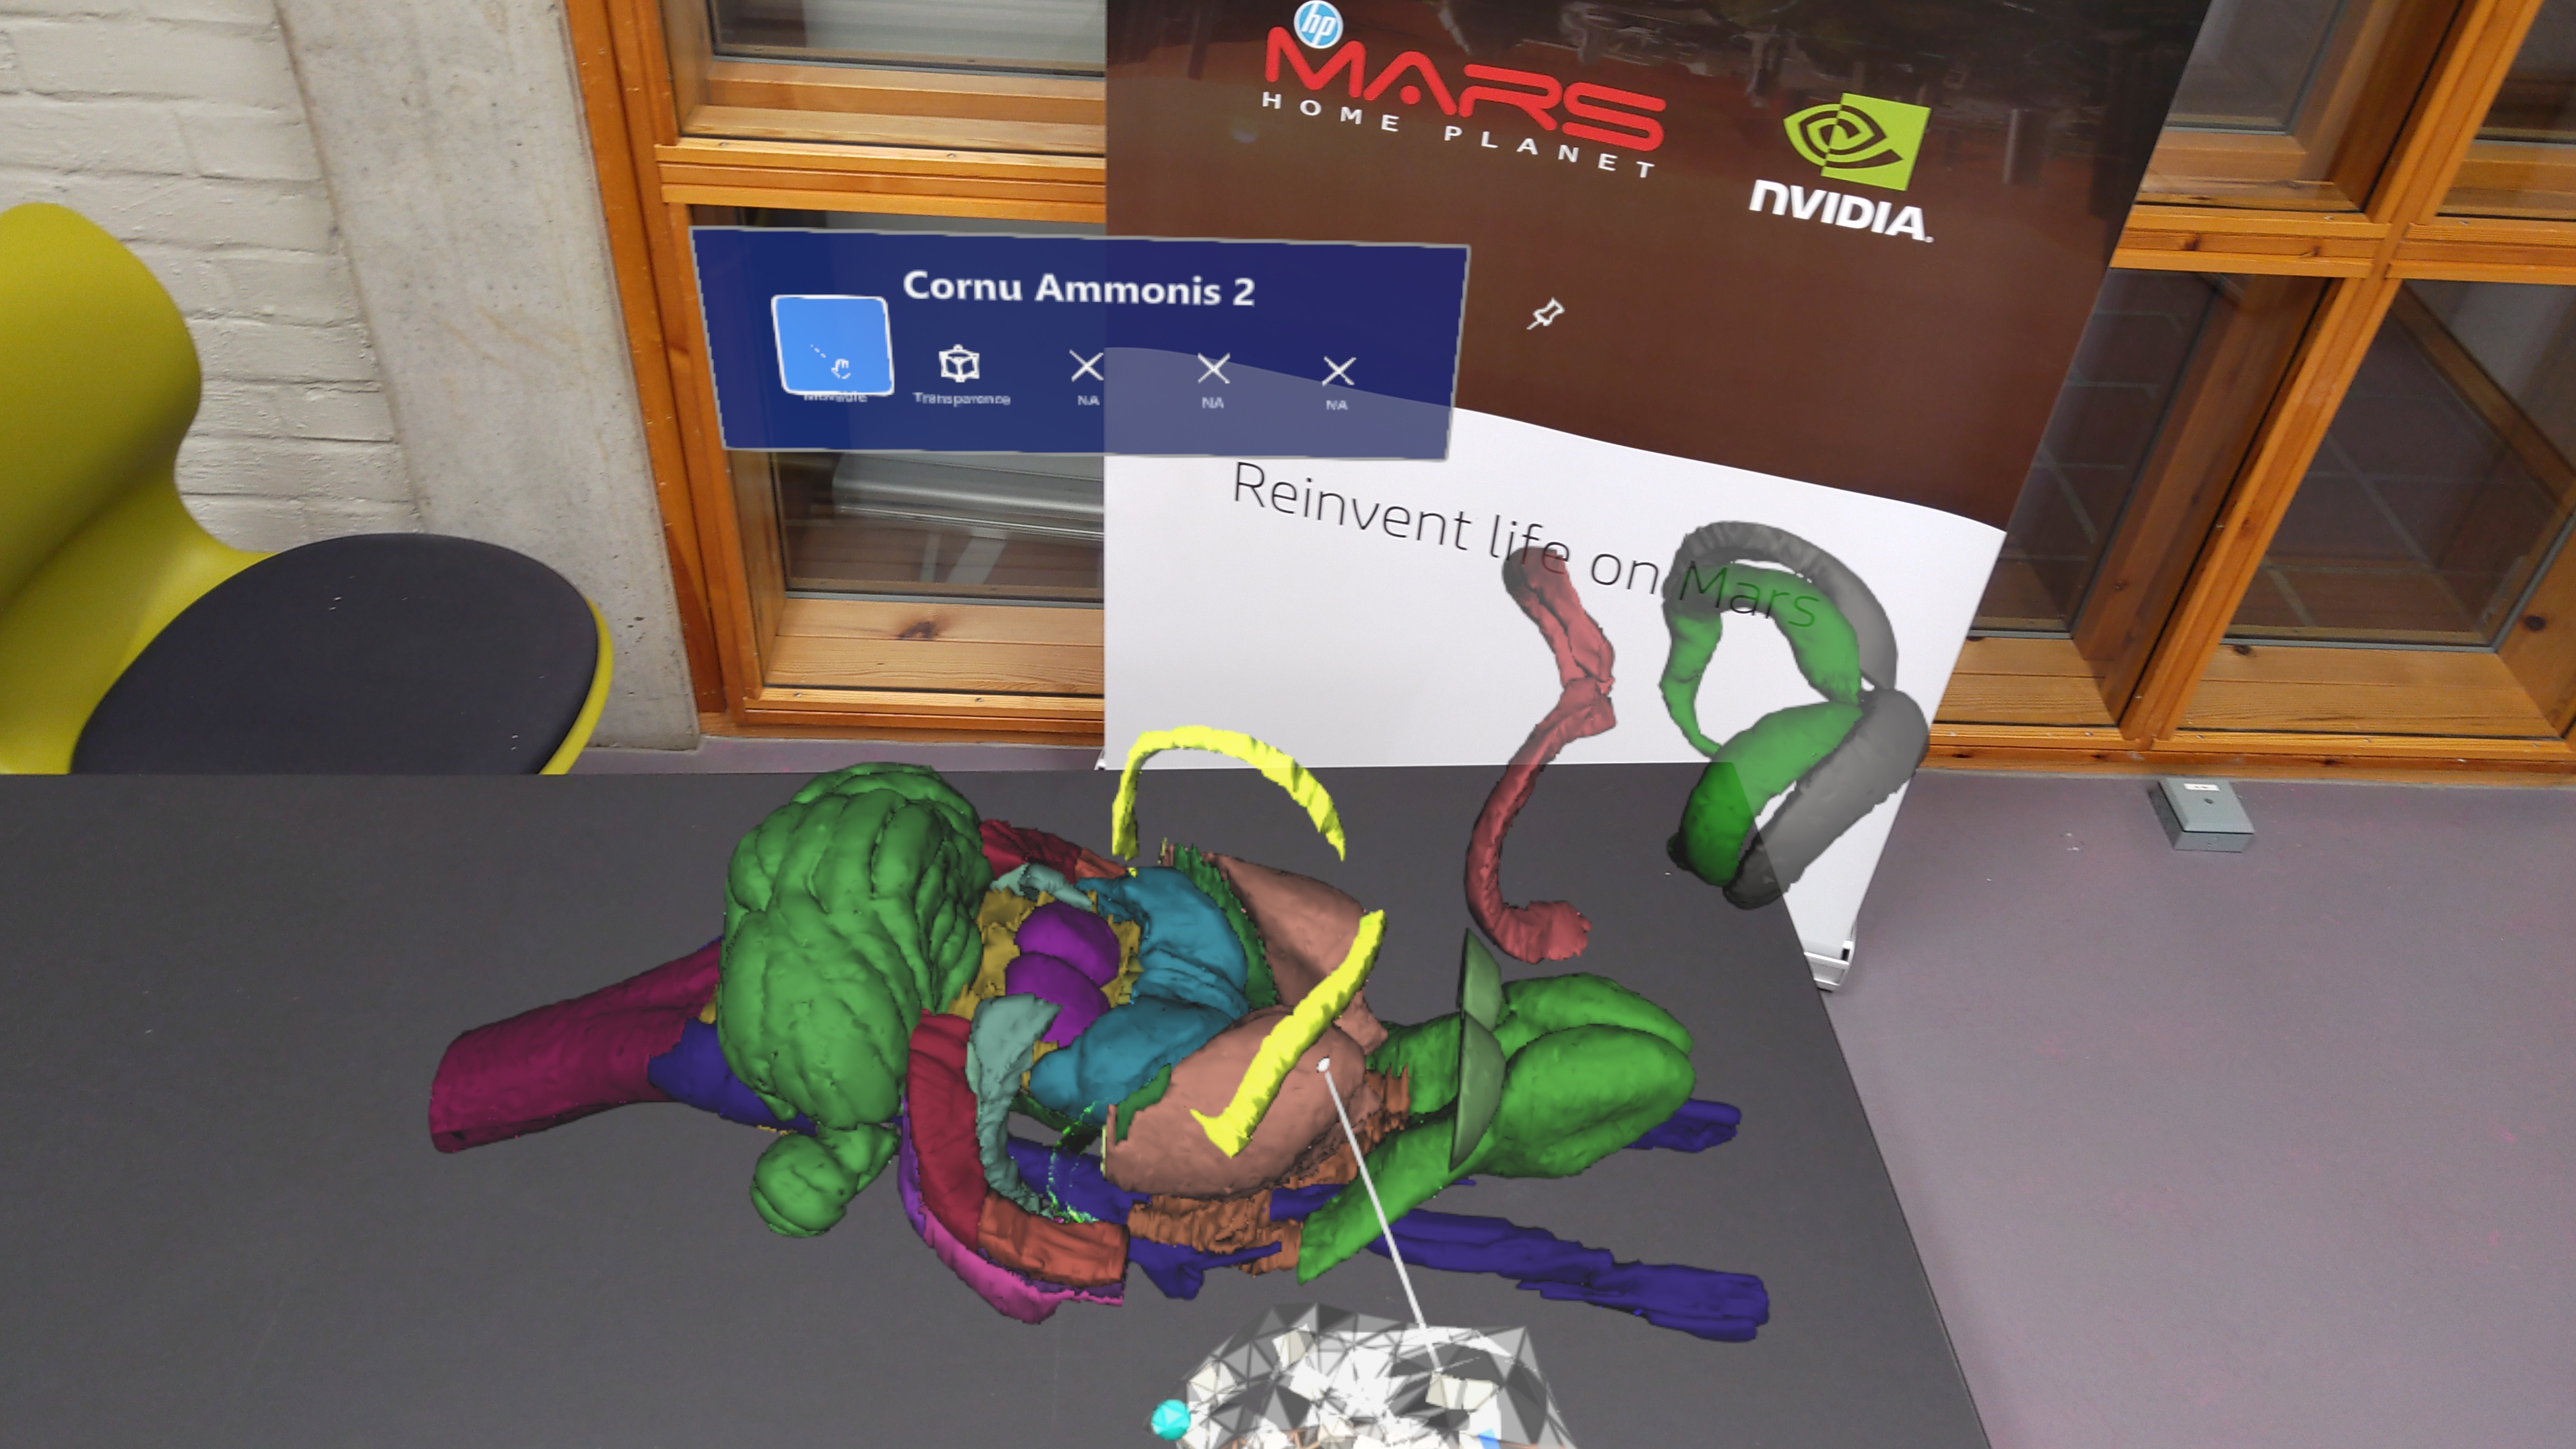
\includegraphics[width=0.5\textwidth]{fig/nevrolens/brainpartsout.jpg}
%     \caption{Nevrolens v0.1.3 on HoloLens 2}
% \end{figure}


% \begin{figure}[h]\label{fig:nevrolens_android}
%     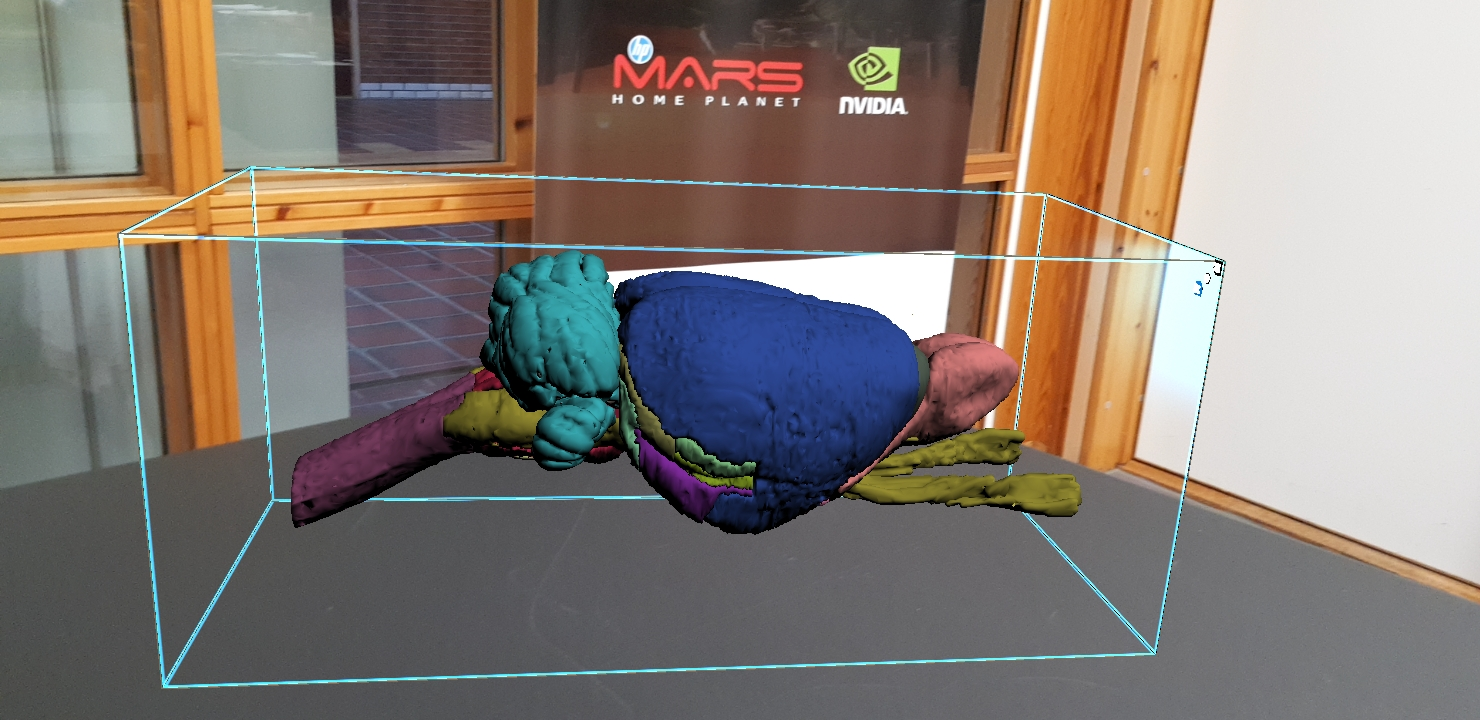
\includegraphics[width=0.5\textwidth]{fig/nevrolens/android_zoom_large.jpg}
%     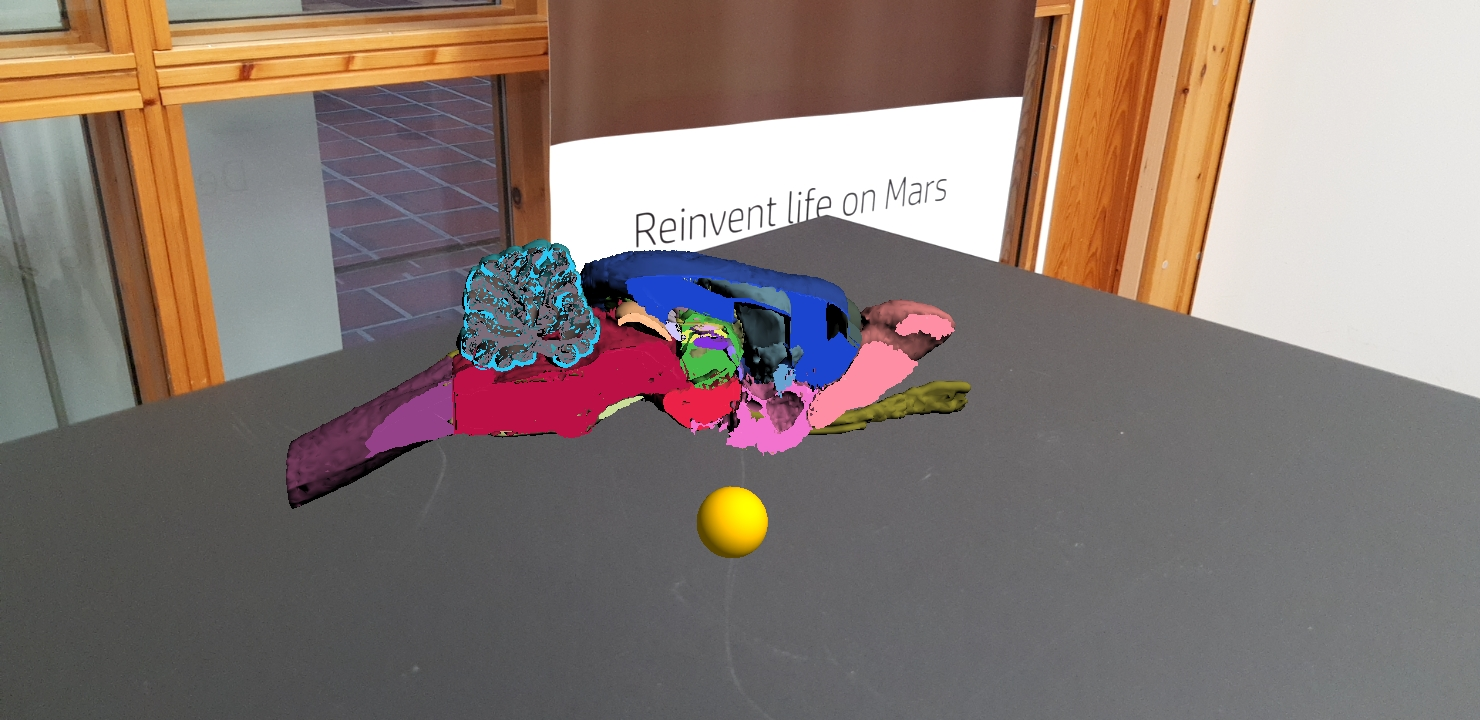
\includegraphics[width=0.5\textwidth]{fig/nevrolens/android_clipping.jpg}
%     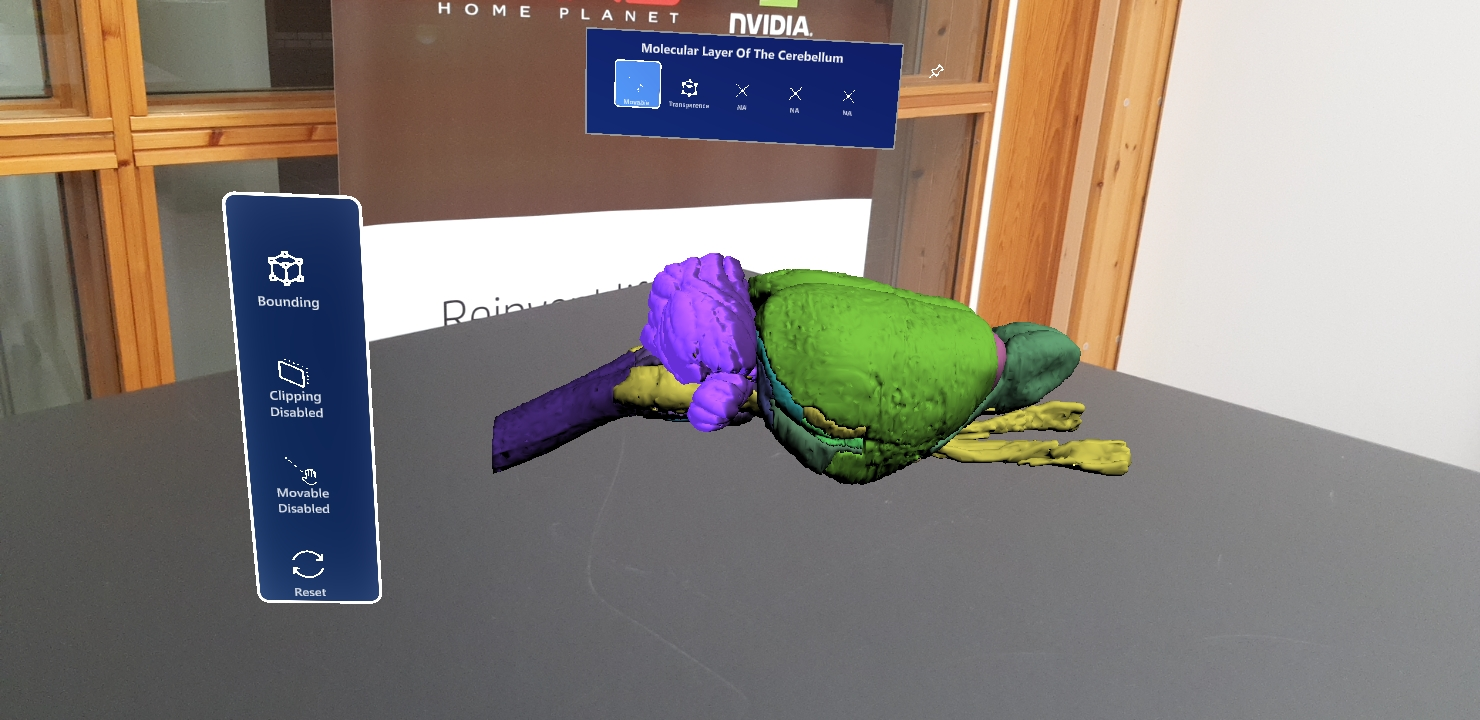
\includegraphics[width=0.5\textwidth]{fig/nevrolens/android_palmmenu.jpg}
%     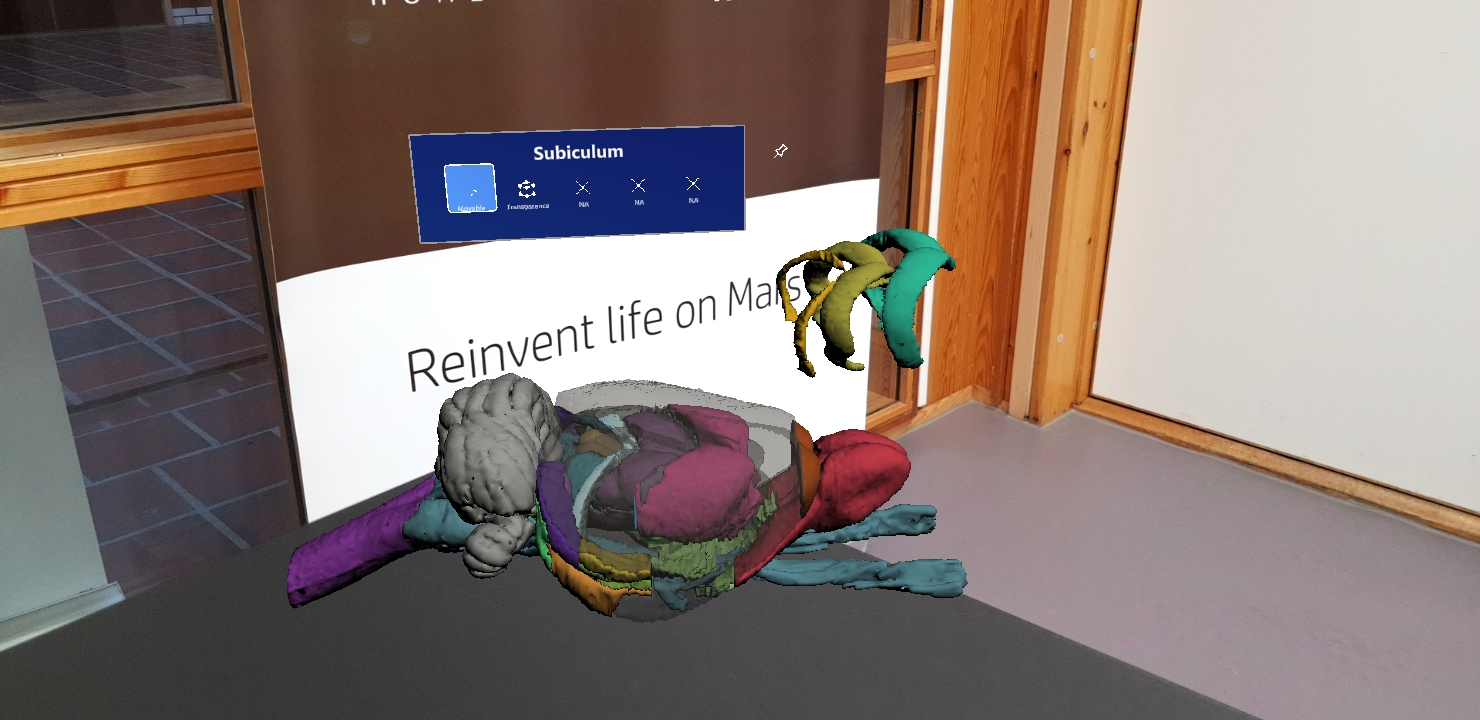
\includegraphics[width=0.5\textwidth]{fig/nevrolens/android_partsout.jpg}
%     \caption{Nevrolens v0.1.3 on Android}
% \end{figure}





% \section{Results}

% Because of the COVID-19 pandemic no user testing has been done this semester, in fact no medical students or professionals have tried the application in-person. Thus, it has been difficult to do formal interviews or gather much feedback, especially regarding interaction. This project is the preliminary work for my master thesis next semester and result gathering will naturally be a much more in focus then. And though no user testing has found place, we have arranged live demoes with \nameref{chap:wdp} over Zoom, which have generated useful feedback. 
% In one such demonstration, I wore a HoloLens 2 and use Nevrolens with guidance from a neuroscientist to extract related regions of the brain and was lectured on their role in behavior. 
% The feedback on its use for a single user, was that there should be a global list menu to toggle different features on each brain part, that there should be ability to increase resolution of a single brain part and some way to visualize microscopical data. 

% % Mostly, the feedback has been positive

% % Success in picking out brain parts, and explaining different structures in the brain. 



% % results from this project are limited.